\documentclass{standalone}

% put this in your preamble
\usepackage{tikz}

\begin{document}
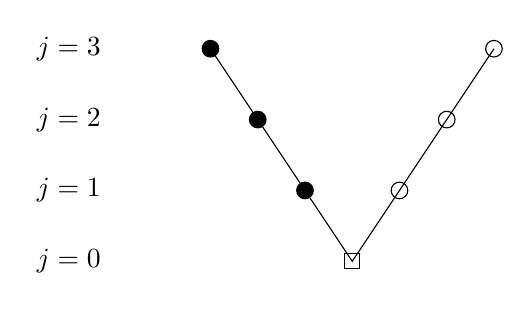
\begin{tikzpicture}[scale=1.2]
  \pgfmathsetmacro\hstep{0.5}
  \pgfmathsetmacro\vstep{0.75}
  \pgfmathsetmacro\ceps{0.08}   % size of square for coarse grid

% grid labels at left
  \node at (-2,3*\vstep) {$j=3$};
  \node at (-2,2*\vstep) {$j=2$};
  \node at (-2,\vstep) {$j=1$};
  \node at (-2,0.0) {$j=0$};

% V-cycle
  \draw[black,thin] (-\hstep,3*\vstep) -- (0.0,2*\vstep) -- (\hstep,\vstep) --  (2*\hstep,0.0)
                    -- (3*\hstep,\vstep) -- (4*\hstep,2*\vstep) -- (5*\hstep,3*\vstep);
  \filldraw (-\hstep,3*\vstep) circle (2.5pt);
  \filldraw (0.0,2*\vstep) circle (2.5pt);
  \filldraw (\hstep,\vstep) circle (2.5pt);
  \draw     (2*\hstep-\ceps,-\ceps) rectangle (2*\hstep+\ceps,+\ceps);
  \draw     (3*\hstep,\vstep) circle (2.5pt);
  \draw     (4*\hstep,2*\vstep) circle (2.5pt);
  \draw     (5*\hstep,3*\vstep) circle (2.5pt);
\end{tikzpicture}
\end{document}
